%%%%%%%%%%%%%%%%%%%%%%%%%%%%%%%%%%%%%%%%%
% Short Sectioned Assignment
% LaTeX Template
% Version 1.0 (5/5/12)
%
% This template has been downloaded from:
% http://www.LaTeXTemplates.com
%
% Original author:
% Frits Wenneker (http://www.howtotex.com)
%
% License:
% CC BY-NC-SA 3.0 (http://creativecommons.org/licenses/by-nc-sa/3.0/)
%
%%%%%%%%%%%%%%%%%%%%%%%%%%%%%%%%%%%%%%%%%

%----------------------------------------------------------------------------------------
%	PACKAGES AND OTHER DOCUMENT CONFIGURATIONS
%----------------------------------------------------------------------------------------

\documentclass[paper=a4, fontsize=11pt]{scrartcl} % A4 paper and 11pt font size

\usepackage[T1]{fontenc} % Use 8-bit encoding that has 256 glyphs
\usepackage{fourier} % Use the Adobe Utopia font for the document - comment this line to return to the LaTeX default
\usepackage[english]{babel} % English language/hyphenation
\usepackage{amsmath,amsfonts,amsthm} % Math packages
\usepackage{graphicx}
\usepackage{lipsum} % Used for inserting dummy 'Lorem ipsum' text into the template
\usepackage{listings}
\usepackage{color}

\definecolor{dkgreen}{rgb}{0,0.6,0}
\definecolor{gray}{rgb}{0.5,0.5,0.5}
\definecolor{mauve}{rgb}{0.58,0,0.82}

\lstset{frame=tb,
  language=Matlab,
  aboveskip=3mm,
  belowskip=3mm,
  showstringspaces=false,
  columns=flexible,
  basicstyle={\small\ttfamily},
  numbers=none,
  numberstyle=\tiny\color{gray},
  keywordstyle=\color{blue},
  commentstyle=\color{dkgreen},
  stringstyle=\color{mauve},
  breaklines=true,
  breakatwhitespace=true,
  tabsize=3
}

\usepackage{sectsty} % Allows customizing section commands
\allsectionsfont{\normalfont} % Make all sections centered, the default font and small caps
\usepackage{fancyhdr} % Custom headers and footers
\pagestyle{fancyplain} % Makes all pages in the document conform to the custom headers and footers
\fancyhead{} % No page header - if you want one, create it in the same way as the footers below
\fancyfoot[L]{} % Empty left footer
\fancyfoot[C]{} % Empty center footer
\fancyfoot[R]{\thepage} % Page numbering for right footer
\renewcommand{\headrulewidth}{0pt} % Remove header underlines
\renewcommand{\footrulewidth}{0pt} % Remove footer underlines
\setlength{\headheight}{13.6pt} % Customize the height of the header

\numberwithin{equation}{section} % Number equations within sections (i.e. 1.1, 1.2, 2.1, 2.2 instead of 1, 2, 3, 4)
\numberwithin{figure}{section} % Number figures within sections (i.e. 1.1, 1.2, 2.1, 2.2 instead of 1, 2, 3, 4)
\numberwithin{table}{section} % Number tables within sections (i.e. 1.1, 1.2, 2.1, 2.2 instead of 1, 2, 3, 4)

\setlength\parindent{0pt} % Removes all indentation from paragraphs - comment this line for an assignment with lots of text

%----------------------------------------------------------------------------------------
%	TITLE SECTION
%----------------------------------------------------------------------------------------

\newcommand{\horrule}[1]{\rule{\linewidth}{#1}} % Create horizontal rule command with 1 argument of height

\title{	
\normalfont \normalsize 
\textsc{CSIT 5210 Data Mining and Knowledge Discovery} \\ [25pt] % Your university, school and/or department name(s)
\horrule{0.5pt} \\[0.4cm] % Thin top horizontal rule
\huge Assignment 1 \\ % The assignment title
\horrule{2pt} \\[0.5cm] % Thick bottom horizontal rule
}

\author{GUO, Yuchen No. 20477118} % Your name

\date{\normalsize\today} % Today's date or a custom date

\begin{document}

\maketitle % Print the title

%----------------------------------------------------------------------------------------
%	PROBLEM 1
%----------------------------------------------------------------------------------------

\section{Data Preprocessing}


%------------------------------------------------

\subsection{Wavelet Transform}

%------------------------------------------------

\subsubsection{Describe the discrete wavelet transform}

\begin{enumerate}
    \item Find the $\frac{p_1+p_2}{\sqrt{2}}$ value of each pair $p_1, p_2$ of samples. Fill the first half of the array with the values.
    \item Find the $\frac{p_1-p_2}{\sqrt{2}}$ value of each pair $p_1, p_2$ of samples. Fill the second half of the array with the values.
    \item Repeat the process on the first half of the array.
\end{enumerate}


\subsubsection{Compute the discrete Haar wavelet transform}

\begin{align*}
& [1, 4, 2, 3, -2, -1, 2, 1]\\ 
\Rightarrow & [\frac{5}{\sqrt{2}}, \frac{5}{\sqrt{2}}, -\frac{3}{\sqrt{2}}, \frac{3}{\sqrt{2}}], [-\frac{3}{\sqrt{2}}, -\frac{1}{\sqrt{2}}, -\frac{1}{\sqrt{2}}, \frac{1}{\sqrt{2}}]\\ 
\Rightarrow & [5, 0], [0, -3]\\ 
\Rightarrow & [\frac{5}{\sqrt{2}}], [\frac{5}{\sqrt{2}}]\\ 
\end{align*}

%----------------------------------------------------------------------------------------
%	PROBLEM 2
%----------------------------------------------------------------------------------------

\subsection{Principal Components Analysis}

%------------------------------------------------

\subsubsection{Calculate the covariance matrix of data as shown in the Table 1.}

The code is:\\

\begin{lstlisting}
X = [-1 -2 -3 1 2 3 1; -1 -1 -2 1 1 2 2; 1 4 -2 1 2 1 4];
covariance = cov(X');
\end{lstlisting}

The output is:\\

$\begin{bmatrix} 
	4.8095 & 3.2857 & 1.2381\\
	3.2857 & 2.5714 & 1.4762\\
	1.2381 & 1.4762 & 4.2857
\end{bmatrix}$

\subsubsection{Calculate eigenvectors and eigenvalues of the covariance matrix.}

The code is:\\

\begin{lstlisting}
[V, D] = eig(covariance);
\end{lstlisting}

The output is:\\

$V=\begin{bmatrix} 
    0.5484 & 0.4373 & 0.7128\\
	-0.8259 & 0.1499 & 0.5435\\
	 0.1308 & -0.8867 & 0.4434\\
\end{bmatrix}; D=\begin{bmatrix} 
    0.1561 & 0 & 0\\
	0 & 3.4255 & 0\\
	0 & 0 & 8.0851\\
\end{bmatrix}$\\

So the eigenvectors are: $[0.5484, -0.8259, 0.1308]^T; [0.4373, -0.1499, 0.8867]^T; [0.7128, -0.5435, 0.4434]^T$.\\

And the corresponding eigenvalues are $0.1561, 3.4255, 8.0851$.

\subsubsection{Calculate the proportion of total population variance explained by the first two components.}

\begin{align*}
    \lambda_1 = 0.1561\\
    \lambda_2 = 3.4255\\
    \lambda_3 = 8.0851\\
\end{align*}


The proportion is: 

\begin{align*}
    \frac{\lambda_2 + \lambda_3}{\lambda_1 + \lambda_2 + \lambda_3}=0.9866
\end{align*}

%------------------------------------------------
\section{Pattern Discovery}


\begin{equation*}
    SessionLengthCategory =
    \begin{cases}
      SL1 & \text{if $SessionLength \le 850$}\\
      SL2 & \text{if $850 < SessionLength\le 1433$}\\
      SL3 & \text{if $SessionLength > 1433$}
    \end{cases}
\end{equation*}

\begin{equation*}
    NumWebPageCategory =
    \begin{cases}
      WP1 & \text{if $NumWebPage \le 9$}\\
      WP2 & \text{if $9 < NumWebPage\le 13$}\\
      WP3 & \text{if $13 < NumWebPage\le 25$}\\
      WP4 & \text{if $NumWebPage > 25$}
    \end{cases}
\end{equation*}

\begin{center}
    \begin{tabular}{|l|l|l|l|l|}
      \hline
      Session ID  & Country & Session Length & \#Web Page & Buy\\
      \hline
      1 & NA & SL2 & WP1 & Yes\\
      2 & A & SL3 & WP2 & Yes\\
      3 & E & SL1 & WP4 & Yes\\
      4 & E & SL2 & WP4 & No\\
      5 & NA & SL1 & WP1 & No\\
      6 & A & SL2 & WP3 & Yes\\
      7 & A & SL3 & WP3 & Yes\\
      8 & A & SL1 & WP1 & No\\
      9 & NA & SL3 & WP2 & No\\
      10 & E & SL2 & WP4 & Yes\\
      \hline
    \end{tabular}
\end{center}

A means Asia, NA means North American, E means Europe.

\subsection{Show the major steps to find the frequent patterns using Apriori of the transactions.}

The following two pictures Figure 2.1, Figure 2.2 shows the two steps of finding frequent patterns.

The frequent patterns are: \\
\{A\}, \{E\}, \{NA\}, \{SL1\}, \{SL2\}, \{SL3\}, \{WP1\}, \{WP4\}, \{Yes\}, \{No\}, 
\{A, Yes\}, \{E, WP4\}, \{SL2, Yes\}.

\begin{figure}[h]
    \centering
    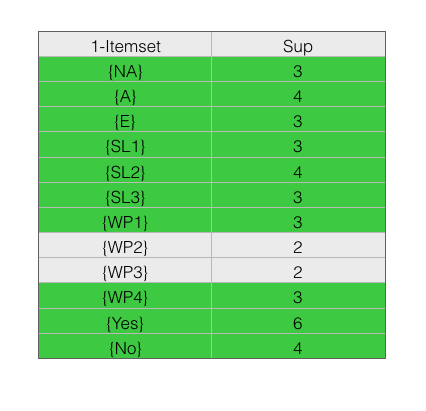
\includegraphics[scale=0.4]{image1.png}
    \caption{Find 1-itemset frequent patterns}
\end{figure}

\begin{figure}[h]
    \centering
    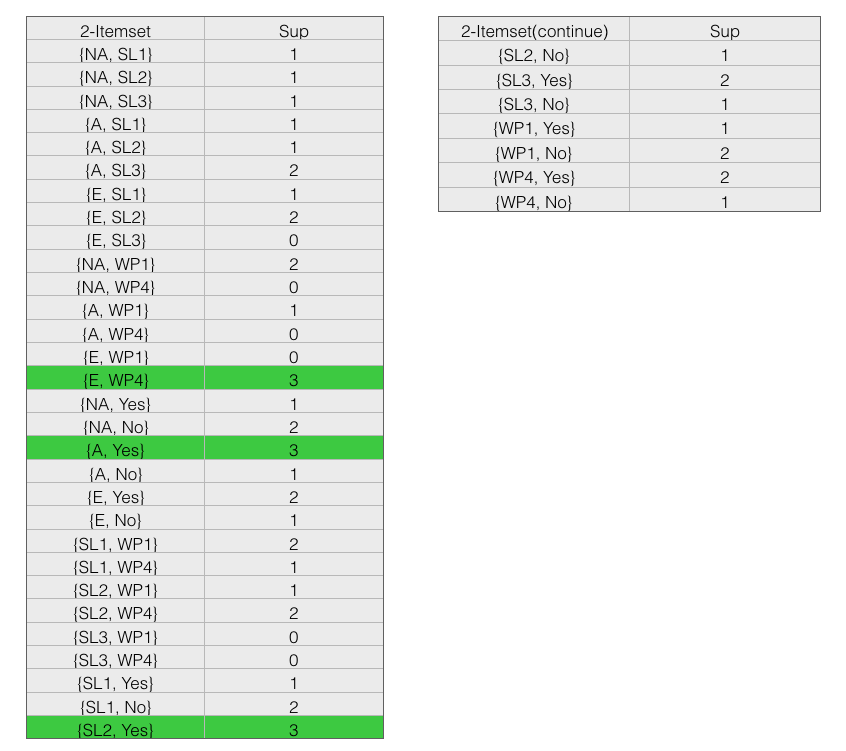
\includegraphics[scale=0.4]{image2.png}
    \caption{Find 2-itemset frequent patterns using Apriori}
\end{figure}

\subsection{Show the major steps to find the frequent patterns using FP-Growth of the transactions.}

Figure 2.3 to Figure 2.8 shows the steps to find fp using FP-Growth.

So frequent items are:
\{A\}, \{E\}, \{NA\}, \{SL1\}, \{SL2\}, \{SL3\}, \{WP1\}, \{WP4\}, \{Yes\}, \{No\}, 
\{Yes, A\}, \{E, WP4\}, \{Yes, SL2\}.

\begin{figure}[h]
    \centering
    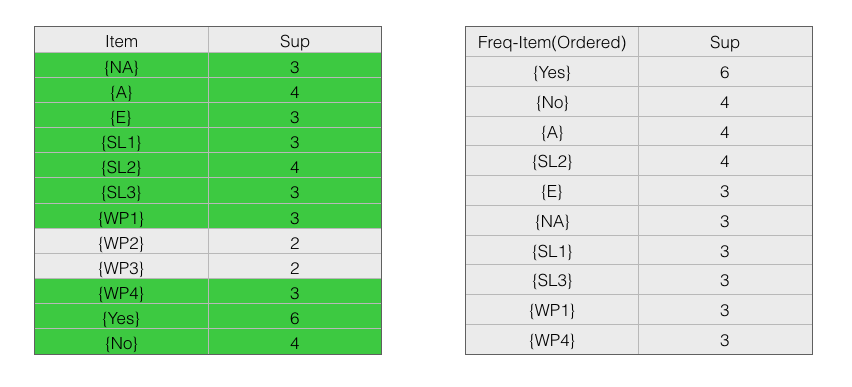
\includegraphics[scale=0.5]{image3.png}
    \caption{Find 2-itemset frequent patterns using FP-tree: Order items}
\end{figure}
\begin{figure}[h]
    \centering
    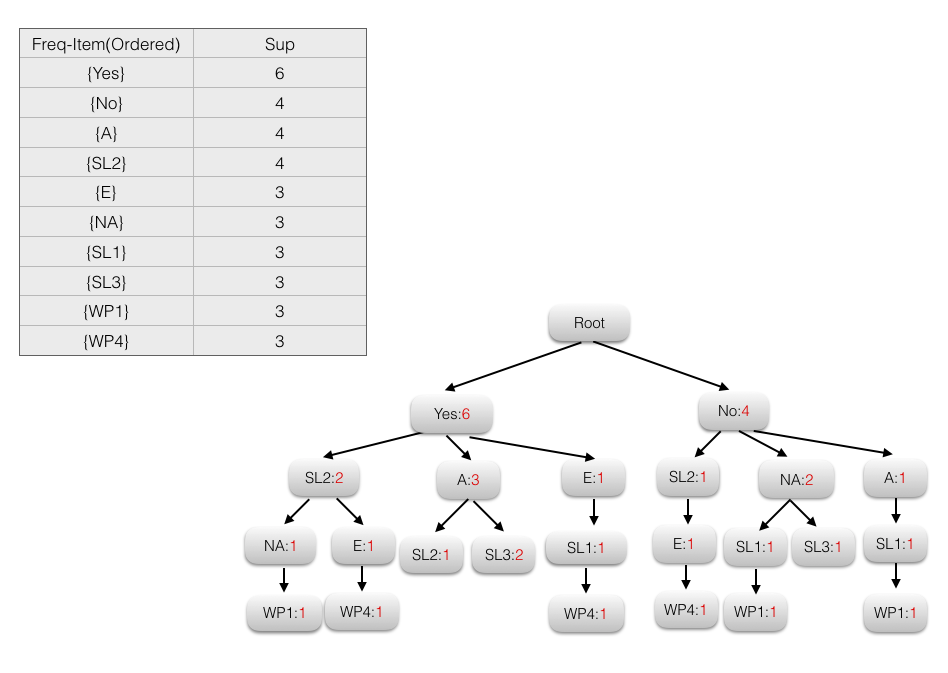
\includegraphics[scale=0.5]{image4.png}
    \caption{Find 2-itemset frequent patterns using FP-tree: Build FP-tree}
\end{figure}
\begin{figure}[h]
    \centering
    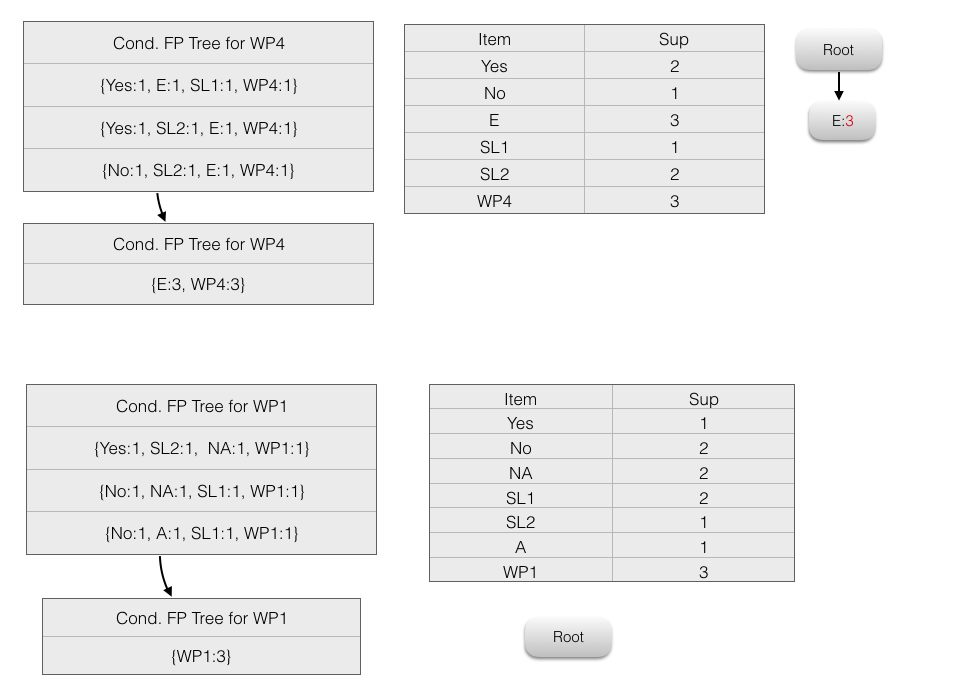
\includegraphics[scale=0.5]{image5.png}
    \caption{Find 2-itemset frequent patterns using FP-tree: Build Cond FP-tree for WP4, WP1}
\end{figure}
\begin{figure}[h]
    \centering
    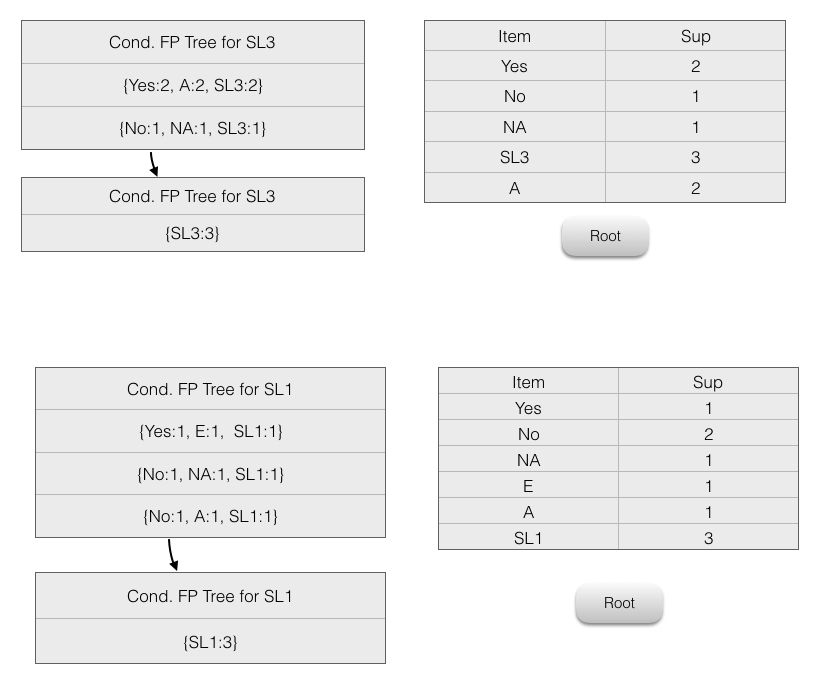
\includegraphics[scale=0.5]{image6.png}
    \caption{Find 2-itemset frequent patterns using FP-tree: Build Cond FP-tree for SL3, SL1}
\end{figure}
\begin{figure}[h]
    \centering
    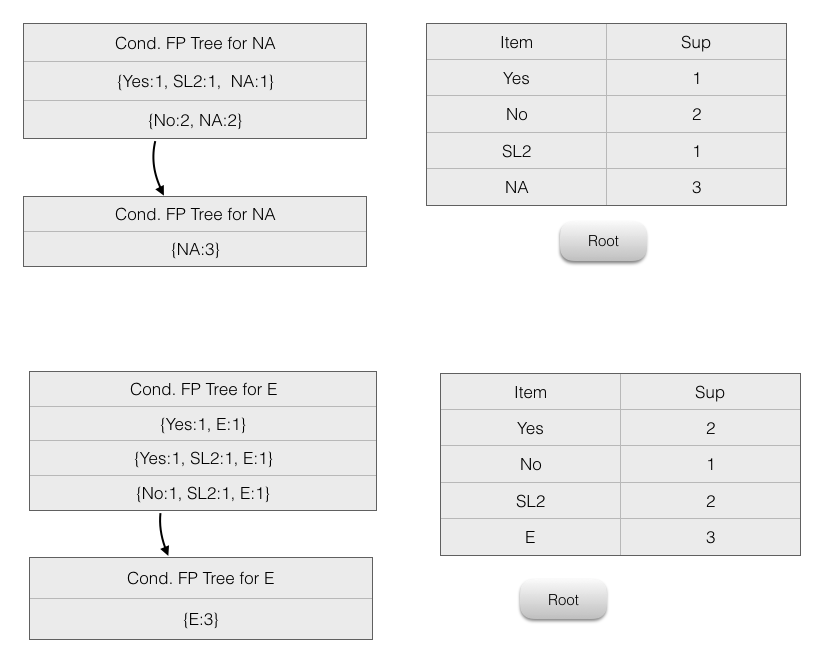
\includegraphics[scale=0.5]{image7.png}
    \caption{Find 2-itemset frequent patterns using FP-tree: Build Cond FP-tree for NA, E}
\end{figure}
\begin{figure}[h]
    \centering
    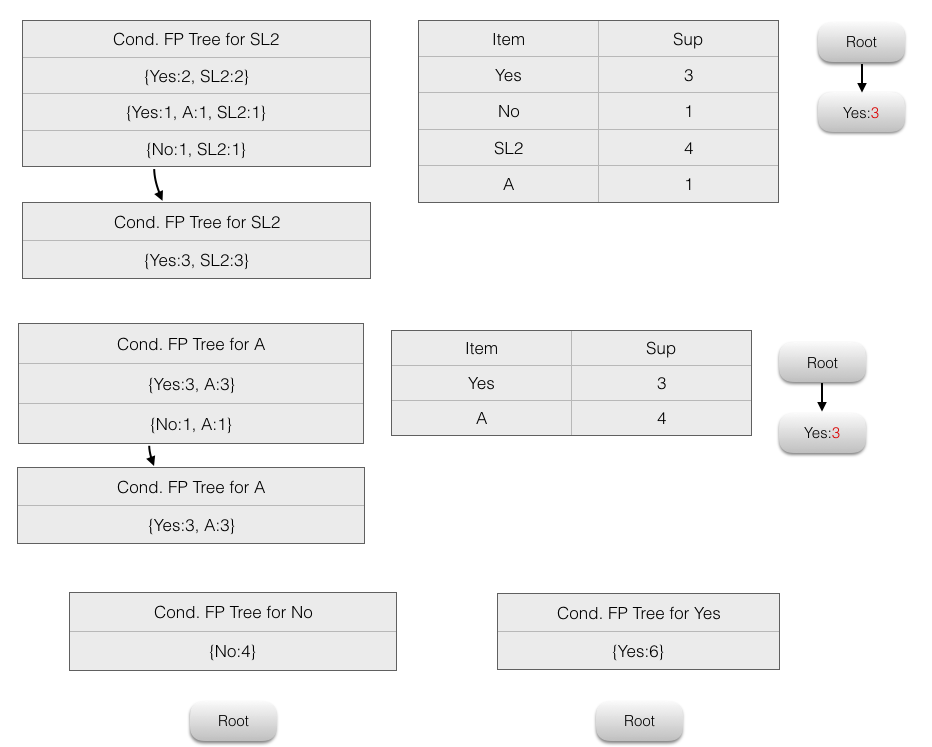
\includegraphics[scale=0.5]{image8.png}
    \caption{Find 2-itemset frequent patterns using FP-tree: Build Cond FP-tree for SL2, A, Yes, No}
\end{figure}

\subsection{Based on the frequent patterns you get, which are closed frequent patterns? Which are max frequent patterns?}

As Figure 2.9 shows:

Closed frequent pattern: \{A\}, \{E\}, \{NA\}, \{SL1\}, \{SL2\}, \{SL3\}, \{WP1\}, \{WP4\}, \{Yes\}, \{No\}, \{Yes, A\}, \{E, WP4\}, \{Yes, SL2\}.

Maximal frequent pattern: \{E\}, \{NA\}, \{SL1\}, \{SL3\}, \{WP1\}, \{WP4\}, \{No\}, \{Yes, A\}, \{E, WP4\}, \{Yes, SL2\}.

\begin{figure}[h]
    \centering
    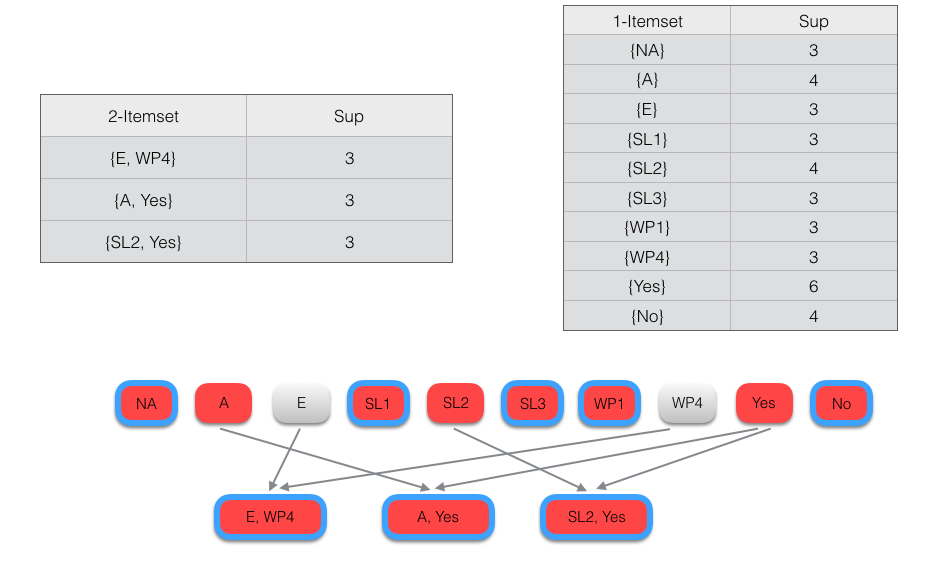
\includegraphics[scale=0.5]{image9.png}
    \caption{Maximal and Closed frequent patterns}
\end{figure}

%----------------------------------------------------------------------------------------

\end{document}